\chapter{Phonological Processes}

In this chapter, we describe the segmental processes in Moro, those that affect vowels, consonants or the interaction between them. 

\section{Consonant-vowel interaction}

\subsection{Palatalization}
Palatalization describes the process whereby consonants are articulated with a palatal off glide [j] (ex. k\super{j}), or shift their articulation to the palatal region, often with a change in manner of articulation. 

The vowel /e/ triggers palatalization of a preceding consonant, adding an off-glide. This affects all consonants except /w/ and /j/. This is an automatic process and will not be indicated in further transcriptions.

\ea
\begin{tabular}[t]{lll}
	élːe	&	[éljːe]		&	‘feather’\\
	ámə́géə	&	[ámə́gjéə] 	&	‘scar’\\
	ðegə́mé	&	[ðjegə́mjé] 	&	‘jaw’\\
	ŋelá	&	[ŋjelá]		&	‘oil’\\
\end{tabular}
\z

The dental stops /t̪/ and /d̪/ are palatalized when followed by the causative suffix \textit{-i}, the passive suffix \textit{-ən}, and the benefactive applicative suffix \textit{-ət̪}, as shown in \tabref{tab:ch5:pal}. Verbs which exceptionally do not show palatalization are given in \tabref{tab:ch5:nopal}. All three suffixes also trigger vowel harmony. No other schwas or [i] trigger palatalization in the language, so this is a lexical process. 

\begin{table}
\begin{tabular}[t]{lllll}
\lsptoprule
&	Perfective	&	Causative perf.	&	Passive perf.	&	Applicative perf.\\
\midrule 
‘lick’	&	k-a-təŋat̪-ó	&	k-ɜ-təŋɜʧ-í	&	kɜ-təŋɜʧ-in-ú	&	k-ɜ-təŋɜʤ-it̪-ú\\
‘prep. soil’	&	k-a-rat̪-ó	&	k-ɜ-rɜʧ-í	&	k-ɜ-rɜʧ-in-ú	&	k-ɜ-rɜʤ-it̪-ú\\
‘sew’	&	k-a-wat̪-ó	&	k-ɜ-wɜʧ-í	&	k-ɜ-wɜʧ-in-ú	&	k-ɜ-wɜʤ-it̪-ú\\
‘repair’	&	k-a-dogat̪-ó	&	k-ɜ-dugɜʧ-í	&	k-ɜ-dugɜʧ-in-ú	&	k-ɜ-dugɜʤ-it̪-ú\\
‘tend’	&	k-a-rəmwət̪-ó	&	k-ɜ-rəmwəʧ-í	&	k-ɜ-rəmwəʧ-in-ú	&	k-ɜ-rəmwəʤ-it̪-ú\\
‘find’	&	k-a-wːaðat̪-ó	&	k-ɜ-wːɜðɜʧ-í	&	k-ɜ-wːɜðɜʧ-in-ú	&	k-ɜ-wːɜðɜʤ-it̪-ú\\
‘watch’	&	k-a-wəndat̪-ó	&	k-ɜ-wəndɜʧ-í	&	k-ɜ-wəndɜʧ-in-ú	&	k-ɜ-wəndɜʤ-it̪-ú\\
‘jump’	&	k-ogət̪-ó	&	k-ugəʧ-í	&	----		&	k-ugəʤ-it̪-ú\\
‘throw’	&	k-ɜwut̪-ú	&	k-ɜwuʧ-í	&	k-ɜwuʧ-in-ú	&	k-ɜwuʤ-it̪-ú\\
‘enter’	&	k-ənt̪-ú	&	k-ənʧ-í	&	k-ənʧ-in-ú	&	k-ənʤ-it̪-ú\\
‘dance’	&	k-a-ɾət̪-ó	&	k-ɜ-ɾəʧ-í	&	---	&	k-ɜ-ɾəʤ-it̪-ú\\
‘close’	&	k-a-land̪-ó	&	k-ɜ-lɜnʤ-í	&	k-ɜ-lɜnʤ-in-ú	&	k-ɜ-lɜnʤ-it̪-ú\\
‘send’	&	k-a-d̪oat̪-ó	&	k-ɜ-d̪uɜʧ-í	&	k-ɜ-d̪uɜʧ-in-ú	&	k-ɜ-d̪uɜʤ-it̪-ú\\
\lspbottomrule
\end{tabular}
\caption{Palatalization triggered by extension suffixes} \label{tab:ch5:pal}
\end{table}

\begin{table}
\caption{Exceptions with no palatalization}\label{tab:ch5:nopal}
\begin{tabular}[t]{lllll}
\lsptoprule
&	Perfective	&	Causative perf.	&	Passive perf.	&	Applicative perf.\\
\midrule
‘drink’	&	kɜ-t̪-ú	&	kɜ-t̪-í	&	kɜ-t̪-ən-ú	&	kɜ-t̪-ət̪-ú\\
‘cough’	&	kɜ-t̪und̪-ú	&	kɜ-t̪und̪-í	&	-----	&	kɜ-t̪und̪-ət̪-ú\\
‘plant’	&	ka-kad̪-ó	&	kɜ-kɜd̪-í	&	kɜ-kɜd̪-ən-ú	&	kɜ-kɜd̪-ət̪-ú\\
\lspbottomrule
\end{tabular}
\end{table}

If the passive suffix follows the applicative, it can trigger palatalization of the applicative: \textit{k-ɜnd-iʧ-in-ú} ‘it was caught for’.

Other sequences of [t̪] or [d̪] followed by [i] do not show palatalization:

\ea
\begin{tabular}[t]{llll}
	ðɜ́ŕt̪í	&	‘anus’	&	uməɾt̪ín	&	‘co-wife’\\
	it̪əlí	&	‘year’	&	id̪əvíní	&	‘shoe’\\
	kɜt̪iðú	&	‘s/he threaded’
\end{tabular}
\z

The proximal subordinate suffix \textit{–i} (a raised version of /-e/) does not palatalize a preceding dental stop, whether that stop is root-final, or is in the applicative affix (c).

\ea
\begin{tabular}[t]{llll}
&	Perfective	&	Subordinate\\
a.&	k-ənt̪-ú		&	... ɜ́ŋ-ə́nt̪-i		&	‘enter’\\
b.&	k-ɜwut̪-ú	&	... ɜ́ŋ-ɜwút̪-i	&	‘throw’\\
c.&	kɜ-kɜd̪-ət̪-ú	&	... ɜ́ŋə́-kɜ́d̪-ə́t̪-i	&	‘plant for’\\
\end{tabular}
\z

The proximal imperfective diphthong suffix \textit{-iə}, which occurs with roots with high vowels, also does not condition palatalization:

\ea
\begin{tabular}[t]{llll}
a.&		kɜt̪úrt̪iə	&	‘s/he is waiting’\\
b.& 	kɜvɜ́ńt̪iə	&	‘s/he is entering’\\
c.&		kɜɾə́mə́ðit̪iə	&	‘s/he is filling a hole’\\
\end{tabular}
\z

The consecutive imperfective complementizer prefix \textit{t̪-́ } occurs word-initially and is also never palatalized, even when followed by the 1st person subject prefix \textit{i-}:

\ea
\begin{tabular}[t]{llll}
a.&		t̪-í-við-ú	&	‘and I vomited’\\
b.&		t̪-í-t̪und̪-ú	&	‘and I coughed’\\
\end{tabular}
\z

In addition to vowels affecting consonants, palatal consonants can also affect vowels. Before the alveopalatal affricates [tʃ] and [dʒ], /a/ is articulated with a palatal off-glide [j]:

\ea
\begin{tabular}[t]{lll}
labatʃó	&	[labajtʃó]	&	‘they lifted’\\
áʧə́vá(ŋ)	&	[ájʧə́váŋ]	&	‘sorghum porridge, food’\\
gadʒə́vá	&	[kajdʒə́vá]	&	‘s/he doesn’t know’\\
\end{tabular}
\z

\subsection{Rounding}
The short central vowels [ə] and [ɘ] are rounded when followed by a labialized consonant, but not in all cases. Consider the following verb paradigms. The labialization of the final root consonant is suppressed before an \textit{-o} or \textit{-u} suffix, but appears to transfer to the vowel of the root in the imperative (9)a-f. However, if there is no labialized consonant, no rounding occurs (9)g-h.

\ea
\begin{tabular}[t]{lllll}
&	imperfective	&	perfective	&	imperative	&\\
a.	&	g-abə́ɾʷ-a	&	g-abəɾ-ó	&	ábə́ɾ-ó	&	‘fly’\\
b.	&	g-abə́t̪ʷ-a	&	g-abət̪-ó	&	ábot̪-ó	&	‘climb up’\\
c.	&	g-ɜ-bə́gw-ɜ	&	g-ɜ-bəg-ú	&	búg-ú	&	‘hit’\\
d.	&	g-ɜ-də́ɾw-ɜ́	&	g-ɜ-dəɾ-ú	&	dúɾ-ú	&	‘stop, stand’\\
e.	&	g-ɜ-tʃə́ndəŋw-ɜ	&	g-ɜ-tʃəndəŋ-ú	&	tʃə́ndúŋ-ú	&	‘go down’\\
f.	&	g-ɜ-múŕkw-ɜ	&	g-ɜ-murk-ú	&	múrk-ú	&	‘roll, slide’\\
g.	&	g-a-bə́ɾ-á	&	g-a-bə́ɾ-ó	&	bə́ɾ-ó	&	‘touch’\\
h.	&	g-a-tʃə́ð-á	&	g-a-tʃəð-ó	&	tʃə́ð-ó	&	‘chop furniture legs’\\
\end{tabular}
\z
In addition, labialized consonants that appear before [ə] or [ɘ] in the root are realized as [u] in the imperative:

\ea
\begin{tabular}[t]{lllll}
&	imperfective	&	perfective	&	imperative\\
a.	&	g-a-mwə́n-á	&	g-a-mwən-ó	&	mwə́n-ó	&	‘suck, lick’\\
b.	&	g-ɜ-mwə́t̪-ɜ	&	g-ɜ-mwət̪-ú	&	mút̪-ú	&	‘sip’\\
c.	&	g-a-wə́t̪-á	&	g-a-wət̪-ó	&	ót̪ó	&	‘choose’\\
d.	&	g-ɜ-wə́ɾ-ɜ́	&	g-ɜ-wəɾ-ú	&	úɾú	&	‘dig, bury’\\
\end{tabular}
\z

This also accounts for the alternation between [uʤí] ‘man/woman’ (Elyasir’s pronunciation) and [wədʒí] ‘woman’ (Angelo’s pronunciation).

The vowel /ɜ/ is rounded to [ɔ] following and preceding labialized consonants. Phonologically it is transcribed as /wɜ/ (see above), but phonetically, it is pronounced [wɔ]. 

\section{Vowels}
In this section, we outline vowel hiatus resolution and vowel harmony.

\subsection{Vowel hiatus resolution}\label{sec:ch5:hiatus}
When two vowels become adjacent due to morpheme concatenation or across word boundaries, the sequence is repaired by deletion, glide formation, or fusion. Across word boundaries and in the verb/adjective morphology, the first vowel is deleted. In nominal morphology, deletion, glide formation and fusion occurs depending on the nature of the vowels.

\subsubsection{Vowel deletion}
Vowel deletion will be addressed first, beginning with sentences. No matter the quality of the two vowels, the first vowel is always deleted and the second one maintained:
\ea Subject + Verb
\z
\ea Verb + Adverb
\begin{tabular}[t]{lll}
	kadaŋó at̪en	&	[kadaŋát̪en]	&	‘he was quiet’\\
\end{tabular}
\z

\ea Verb + Postposition/particle
\z

\ea Verb + Noun
\begin{tabular}[t]{llll}
a.	&	k-a-wːaðat̪-ó  evəla	&	[kawːaðat̪ évəla]	&	‘he found the wild cat’\\
b.	&	k-a-wːaðat-ó  ugi	&	[kawːaðat̪ úgi]	&	‘he found the tree’\\
c.	&	k-uə́ndit̪-ú evəla	&	[kuə́ndit̪ évəla]	&	‘he listened to the wild cat’\\
d.	&	áŋə́-wːaðat̪-e ugi	&	[áŋə́wːaðat̪ ugi]	&	‘(that) he finds the tree’\\
e.	&	ɜ́ŋə́-wːɜð-i ugi	&	[ɜ́ŋə́wːɜð ugi]	&	‘(that) he makes find the tree’\\
f.	&	ɜ́ŋə́-wːɜð-i ɜt̪úli	&	[ɜ́ŋə́wːɜð ɜt̪úli]	&	‘(that) he makes find the spear’\\
\end{tabular}
\z

Word-internally, the same effect is observed. In examples a-f, the root clause markers \textit{a-/ɜ-}, \textit{é-/í-} delete in favor of the first vowel of the root. In examples g-h, the vowel of the object marker is deleted. 

%\ea
\begin{tabular}[t]{llllll}
a.&	k-a-erl-ó		&	/a-e/&	[e]	&	[kerló]		&	‘he walked’\\
b.&	k-ɜ-ilið-ú		&	/ɜ-i/&	[i]	&	[kiliðú]		&	‘he bought’\\
c.&	k-é-aɾ-ó		&	/é-a/&	[á]	&	[káɾó]		&	‘…who cried’	 \\
d.&	k-é-ogət̪-ó		&	/é-o/&	[ó]	&	[kógət̪ó]	&	‘…who jumped’\\
e.&	k-í-ɜnt̪-ú		&	/í-ɜ/&	[ɜ́]	&	[kɜ́nt̪ú]		&	‘…who entered’\\
f.&	k-í-udən-ú		&	/í-u/&	[ú]	&	[kúdənú]		&	‘…who farted’\\
g.&	k-ɜ-ɲí-ɜwut̪-ú	&	/í-ɜ/&	[ɜ]	&	[kɜ́ɲɜwut̪ú]	&	‘he dropped me’\\
h.&	k-ɜ-ŋɜ́-ilið-ət̪-ú&	/ɜ́-i/&	[i]	&	[kɜ́ŋiliðət̪ú]&	‘he bought for you’\\
\end{tabular}
%\z

\subsubsection{Glide formation}
The locative affix \textit{–ánó} triggers glide formation if the first vowel is peripheral /i e u o/ (15)a-d, but vowel deletion if it is central /ə ɜ a/ (15)e-g.

\ea
\begin{tabular}[t]{llllll}
a.&	ðugi-ánó	&	/i-á /	&	[já]&	[ðugjánó]	&	‘inside the plank’\\
b.&	ome-ánó		&	/i-á / 	&	[já]&	[omjánó]		&	‘inside the fish’\\
c.&	umu-ánó		&	/u-á/	&	[wá]&	[umwánó]		&	‘inside the Arab (derog.)’\\
d.&	ŋombogó-ánó	&	/o-á/	&	[wá]&	[ŋombogwánó]&	‘inside the calf’\\
e.&	utɾə-ánó	&	/ə-á/	&	[á]	&	[utɾánó]	&	‘inside the pig’\\
f.&	ɜwíɾɜ-ánó	&	/ɜ-á/	&	[á]	&	[ɜwíɾánó]	&	‘inside the tree sp.’\\
g.&	aŋorá-ánó	&	/á-á		&	[á]	&	[aŋoránó]	&	‘inside the elephant’\\
\end{tabular}
\z

% TODO Data When this marker appears on the verb in verb + particle combinations the same effects are observed.

\subsubsection{Vowel fusion}
The demonstrative suffix \textit{-íCːi} (C = noun class concord consonant) shows reduction to [ə] with peripheral vowels (16)a-d or vowel fusion with central vowels (16)e-f.

\ea
\begin{tabular}[t]{llllll}
a.&	ðugi-íðːi	&	/i-í/&	[ə́]	&[ðugə́ðːi]	&‘this plank’\\
b.&	ome-íkːi	&	/e-í/&	[ə́]	&[omə́kːi]	&‘this fish’\\
c.&	ɜðu-ísːi	&	/u-í/&	[ə́]	&[ɜðə́sːi]	&	‘this breast’\\
d.&	ŋombogó-íŋːi&	/ó-í/&	[ə́]	&[ŋombogə́ŋːi]&	‘this calf’\\
e.&	ðuwːɜ-íðːi	&	/ɜ-í/&	[ɜ́]	&[ðuwɜ́ðːi]	&‘this smoke’\\
f.&	ðapa-íðːi	&	/a-í/&	[ɜ́]	&[ðapɜ́ðːi]	&‘this friend’\\
\end{tabular}
\z

It is hard to tell which vowel has been deleted since all peripheral vowels may reduce to [ə] (Gibbard et al 2009). When V1 is central, however, vowel fusion appears to take place, producing a central, but raised [ɜ].

\subsection{Vowel reduction}\label{sec:ch5:vreduction}
The high vowels /i u/ centralize and reduce to [ɘ] and the mid vowels /e o/ may reduce to [ə]; they are both transcribed here as [ə]. Vowel reduction is variable, but occurs between consonants. It is often triggered by the addition of affixes, but may also occur across words, particularly in the verb - object configuration.

\ea Between words
\begin{tabular}[t]{ll}
kaɾənó ŋáwá  $\rightarrow$ [kaɾənə́ ŋáwá]	&	‘s/he swallowed water’\\
\end{tabular}
\z

Singular forms that begin with one of the vowels /i e u o/ show reduction to [ə] with the addition of a plural prefix /n-/:

\ea
\begin{tabular}[t]{llll}
&	singular&	plural\\
a.&	ibəgwɜ́	&	n-əbəgwɜ́	&	‘back of knee’\\
b.&	ebamba 	&	n-əbamba		&	‘drum’\\
c.&	uməní 	&	n-əmwəní 	&	‘tree sp.’\\
d.&	otʃːa 	&	n-ətʃːa 	&	‘milk pot’\\
\end{tabular}
\z

Reduction occurs after the progressive prefix \textit{v-} in (19)a, and locative prefix \textit{ék-/ík-} in (19)b,c. The object marker \textit{ɲé} causes reduction of the preceding vowel /ó/ when attached as a suffix in (19)d, but it reduces itself when attached as a prefix in (19)e.

\ea Affixes
\begin{tabular}[t]{lllll}
  	a.& gilíðɜ \~ gɜvə́líðɜ	&	‘s/he is buying’\\
	b.&	iɾə́ŋ 				&	‘name’	&	ík-əɾə́ŋ		&	‘in name’\\
	c.&	ebamba				&	‘drum’	&	ék-ə́bámbá		&	‘in drum’\\
	d.&	lanatʃó-ɲé lavəðá  	&[lanatʃə́ɲé lavəðá]	&	‘s/he gave me a fig’\\
	e.& la-ɲé-natʃa lavəðá	&[laɲə́natʃa lavəðá]	&	‘s/he is about to give me a fig’\\
\end{tabular}
\z

\subsection{Epenthesis}\label{epenthesis}
The vowel [ə] (or [ɘ] under harmony) is inserted to break up consonant sequences, and to aid in the pronunciation of initial geminates. Some verb roots begin with geminate consonants. When they occur in the imperative with no prefixes, [ə] is inserted before obstruent geminates. There are also some nouns that appear to have epenthetic vowels.

\ea
\begin{tabular}[t]{llll}
Verbs	&	&	Nouns\\
ə́sːó	&	‘eat!’	&	ɘ́sːí	&	‘eye’\\
ɘ́pːú	&	‘beat!	&	ə́rːá	&	‘lizard’\\
ɘ́wːí	&	‘boil!’	&	ɘ́sːiə́	&	‘fire’\\
ə́t̪ːú	&	‘drink!’	&	əwːɜgɜ́	&	‘threshing floor’\\
\end{tabular}
\z

The other case of initial [ə] involves consonant sequences with initial liquids: /rl/ /rm/ /ɽt/ /ln/, /lt/, /lt̪/ and /ld̪/. These sometimes alternate with CəC. They may be considered epenthesis or metathesis (switching of ə and the first consonant). 

\ea
\begin{tabular}[t]{lll}
əCC	&	CəC\\
ə́rl-ó	&	g-a-rə́l-á	&	‘bear fruit/have rash, scabs’\\
ə́rlát̪-ó	&	g-a-rə́lát̪-a	&	‘stomp, trample’\\
ərmeə	&				&	‘rib’\\
ə́ɽtú		&				&	‘gazebo, shade structure\\
əlná	&	lənːá		&	‘room’\\
əltú		&				&	‘shelter’\\
ə́ltóléa		&				&	‘cheek, shouting’\\
əltúr		&				&	‘umbilical hernia’\\
ə́ltə́miə́		&				&	‘barren woman’\\
ə́lt̪ə́miə́		&				&	‘termite mound’\\
ə́ld̪ə́máná		&				&	‘bean’\\
\end{tabular}
\z

Epenthesis also occurs between consonant sequences that arise through morpheme concatenation.

% TODO Sharon INSERT EXAMPLES

\subsection{Vowel harmony}\label{section:vharmony}
Thetogovela Moro has a vowel harmony system that is productive, even applying to loanwords. The ‘lower’ set of vowels /e a o/ raise to the higher counterparts /i ɜ u/ respectively. In addition, phonetic evidence suggests that there are two kinds of schwa, a lower /ə/ which patterns with /e a o/, and its alternate, a higher /ɘ/ that groups with /i ɜ u/ according to harmony (see Ritchart \& Rose 2017 for more details).

Unlike other Kordofanian languages, such as Laru (REF) or Acheron (REF), we have not found evidence for  contrastive distinctions within the same height category, such as /e/ and /ɛ/ or /i/ and /ɪ/, contrasts which are assumed to involve the feature Advanced Tongue Root (ATR).

Vowel height can be measured acoustically by using the first formant. A low first formant (F1) corresponds to a higher vowel, whereas a high F1 corresponds to lower vowel. Vowel backness corresponds to the second formant, or F2; low F2 corresponds to a backer vowel. The mean F1 and F2 values of the vowels for for four speakers (three male, one female) are given below. The higher vowels [i] and [u] have a lower F1 (avg. 330-350Hz)  than their lower mid counterparts [e] and [o] and the mid central vowel [ɜ] (avg. 449-455), a difference of about 100 Hz. The vowel [ɜ] has a lower F1 than the low vowel [a] (avg. 643), a difference of about 200 Hz. Finally, the  central vowel [ɘ] has an F1 slightly higher than the high vowels, by about 20Hz, while the F1 of [ə] is slightly higher than the mid vowels, again by about 20Hz. The difference between the two short central vowels is about 100Hz. 

Mean F1 and F2 values of the vowels 
\begin{table}
  \begin{tabular}{lllll}
    \lsptoprule
	Vowel &	Mean F1 &	Standard Deviation	&	Mean F2 &	Standard Deviation	\\
	\midrule
	i	&   330.4	&	38.6		&	2212.8	&	175.3 \\
	e	&	453.9 	&	66.2		&	2076.2	&	  233.1	\\
	u	&	350.0	&	43.1		&	1025.4	&	280.5	\\
	o	&	449.3 	&	61.9		&	990.7	&	213.0	\\
	ɘ	&	372.3	&	54.9		&	1415.4	&	327.6	\\
	ə	&	479.7 	&	68.3		&	1297.7	&	263.2	\\
	ɜ	&	455.7	&	52.5		&	1711.1	&	255.5	\\
	a	&	642.9 	&	87.0		&	1464.5	&	206.1	\\
\lspbottomrule
  \end{tabular}
  \caption{F1 \& F2 of vowels}
  \label{tab:ch2:2}
\end{table}


The figure shows that [i] has a lower F1 (hence is a ‘higher’ vowel) than [e] and the same goes for the comparison between [u] and [o]. In general, back vowels have higher F1 than front vowels. The mid-front-central vowel [ɜ] has lower F1 than the low-central [a]. The vowel [ɘ] is positioned as a high-mid vowel compared to the high and mid front vowels [i e] and high and mid back vowels [u o. The vowel [ə] is a mid-low vowel compared to the mid vowels [e] [o] and [ɘ] and the low vowel [a]. 

\begin{table}
	\begin{tabular}[t]{llllll}
	\lsptoprule 
Vowel	&	Mean F1	&	Standard Deviation	&	Mean F2	&	Standard Deviation\\
i   	&	293.23	&	25.96	&	2263.32	&	125.49\\
u	&	343.13	&	38.45	&	1042.03	&	166.41\\
ɘ	&	365.21	&	49.03	&	1253.44	&	253.10\\
ɜ	&	414.62	&	50.55	&	1737.46	&	171.09\\
\lspbottomrule 
	\end{tabular}
	\caption{Mean F1 of higher vowels}
	\label{tab:ch5:1}
\end{table} 

\begin{table}
	\begin{tabular}[t]{llllll}
	\lsptoprule 
Vowel	&	Mean F1	&	Standard Deviation	&	Mean F2	&	Standard Deviation\\
e	&	379.67 	&	55.58	&	2030.30	&	85.58\\
o	&	426.08 	&	65.16	&	1068.93	&	133.06\\
ə	&	445.77 	&	44.09	&	1154.88	&	179.26\\
a	&	556.87 	&	74.29	&	1477.02	&	127.66\\
\lspbottomrule 
	\end{tabular}
	\caption{Mean F1 of lower vowels}
	\label{tab:ch5:2}
\end{table} 

\begin{figure}
  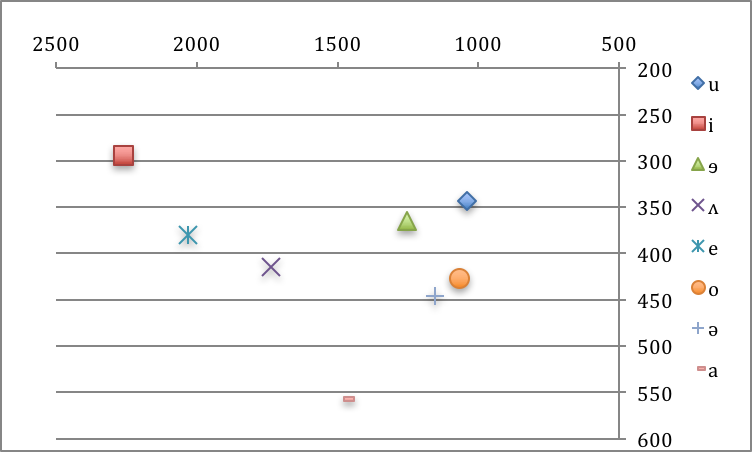
\includegraphics[width=\linewidth]{figures/fig-ch5-1.png}
  \label{fig:5-1}
\end{figure}

The vowel ɜ is acoustically in the mid range, even though it patterns with the higher vowels for the purposes of vowel harmony. Allowing for the fact that back vowels are generally lower than front vowels acoustically, the vowels fit into the basic descriptive categories as follows:

\ea
\begin{tabular}[t]{llll}
&	front	&	central	&	back\\
high	&	i	&	&	u\\
high-mid	&	&	ɘ\\
mid 	&	e	&	ɜ	&	o\\
low-mid	&	&	ə\\
low	&	&	a\\
\end{tabular}
\z

We treat the vowels ə and ɘ as central because they can be subject to some coarticulation. The examples in the above chart were followed by back round vowels, which lowered their F2. 

The vowel harmony system can be understood by examining prefixes and suffixes that alternate depending on harmony. Harmony pervades the nominal and verbal systems. In both, the root controls harmony, but in both systems, there are some suffixes that condition raisin.

\subsubsection{Vowel harmony in noun stems}
Prefixes that attach to nouns harmonize with the vowels of the noun stem. The locative prefix that appears on nouns is a clear example. This prefix may be either [e] or [i] in accordance with the vowels of the noun stem. In these examples, there is a single vowel in the root. If the noun stem contains one of the vowels from the set /e a o ə/, the prefix is [e], whereas if the noun stem contains one the vowels from the set /i ɜ u ɘ/, the prefix is [i]. 

\ea
\begin{tabular}[t]{llllll}
	a.&	é-rló		&	‘in the female goat’		
	&	e.&	í-ltú	&	‘in the shelter’\\
	b.&	é-ðáð		&	‘in the path’		&	f.&	í-ðí	&	‘in the thorn’\\
	c.&	é-ðéj		&	‘in the hand’		&	g.&	í-ɽŕwɜ́	&	‘in the goat manure’\\
	d.&	é-ŋgə́m 		&	‘in the squirrel’	&	h.&	í-ŋgwɘ́ɲ	&	‘in the sign’ \\
\end{tabular}
\z

The locative prefix therefore has two realizations that depend on vowel harmony, and the mid [e] and high [i] can be considered harmonic counterparts. Some examples of longer stems with more vowels are given below (note that the prefix ends in [k] before vowel-initial nouns belong to the g-noun class).

\ea
\begin{tabular}[t]{llllll}
	a.&	é-logopáj		&	‘in the cup’		
	&	e.&	í-ŋwulúð	&	‘in the termites’\\
	b.&	é-ðə́gəmjé		&	‘in the jaw’		&	f.&	ík-id̪ɘvín	&	‘in the shoe’\\
	c.&	é-ŋávəléka		&	‘in the mule’		&	g.&	í-ðɜ́ŋguri	&	‘in the chameleon’\\
	d.&	é-lə́və́ɾá 		&	‘in the stick’	&	h.&	íðɘ́púndrí	&	‘in the wood’ \\
\end{tabular}
\z


All the nouns in the above examples show the same harmonic effect on the prefix. Furthermore, they  are themselves composed of vowels from one of the two harmonic sets. Vowels of the 'lower' set /e a o ə/ cooccur whereas vowels of the 'higher' set /i ɜ u ɘ/ cooccur, and there is little mixing.  

Like the locative prefix, the genitive prefix also harmonizes. This prefix is of the shape Ca- (the C represents noun class agreement) or Cɜ-. The prefix attaches to the possessor, but the consonant agrees with the noun class of the possessed. Whether the possessed has high vowels or not does not affect the pronunciation of the genitive prefix. When the vowels of the possessor are from the lower set (/a e o ə/), the prefix is pronounced with the low vowel [a]:

\ea
\begin{tabular}[t]{lll}
	ajén 	&	ja-ŋálːo	&	‘Ngalo’s mountain’\\
	rápá 	&	ra-ŋálːo	&	‘Ngalo’s friends’\\
	ládéə 	&	la-ŋeɾá		&	‘the girl’s hat’\\
	rápá 	&	ra-ŋeɾá		&	‘the girl’s friends’	\\
	lubə́lbə́líə&	la-ŋeɾá		&	‘the girl’s earlobe’\\
	rɜ́gí 	&	ra-ŋeɾá		&	‘the girl’s wounds’\\
\end{tabular}
\z

When the possessor has a higher vowel, however the genitive prefix is realized with [ɜ]
\ea
\begin{tabular}[t]{lll}
	ajén 	&	jɜ-kúku		&	‘Kuku’s mountain’\\
	rápá 	&	rɜ-kúku		&	‘Kuku’s friends’\\
	ŋádéə 	&	ŋɜ-lɘmːiə	&	‘the boys’ hats’\\
	rápá 	&	rɜ-lɘmːiə	&	‘the boys’ friends’\\
\end{tabular}
\z

There are also some noun class prefixes that harmonize. In general noun class prefixes are consonants, and they are categorized according to the type of consonant. However, Gibbard et al (2009) argue that the j noun class is characterized by vocalic prefixes. The singular has the prefix \textit{a-} and the plural the prefix \textit{e-}, as follows:

\ea
\begin{tabular}[t]{lll}
	singular	&	plural\\
	a-jén 	&	e-jén 	&	‘mountain’\\
	á-ɾómá 	&	é-ɾómá 	&	‘black biting ant’\\
	a-t̪ə́ndŕeá&	e-t̪ə́ndŕeá&	‘cloven hoof’\\
	a-bəl	&	e-bəl	&	‘type of bird that hangs upside down’\\
\end{tabular}
\z

If the root has high vowels, the prefixes are \textit{ɜ-} and \textit{i-} respectively:	

\ea
\begin{tabular}[t]{lll}
	singular	&	plural\\
	ɜ-bulúkriə 	&	i-bulúkriə 	&	‘dove’\\
	ɜ-t̪úmí 		&	i-t̪úmí 		&	‘onion’\\
	ɜ-mwəɾíní	&	i-mwəɾíní	&	‘red-necked cobra’\\
	ɜ-ðú		&	i-ðú			&	‘breast’\\
\end{tabular}
\z

Harmony does not affect most nominal suffixes. The instrumental or comitative suffix \textit{–Ca} agrees for noun class with the noun to which it attaches and has the same tone as the final syllable of the noun stem. However, it does not undergo vowel harmony. This is in clear contrast with the genitive \textit{Ca-} prefix, which takes the same segmental shape.

\ea
\begin{tabular}[t]{lll}
	nəbamba-na	&	‘with the drums’	ɜt̪úlɜ-ja	&	‘with the big spear’\\
	áróm-já		&	‘with the anthill’	lɜmí-lá	&	‘with the beard’\\
	emərt̪á-gá	&	‘with the horse’	ŋusí-ŋá		&	‘with the chick’\\
\end{tabular}
\z

The demonstrative suffix is \textit{–íCːi}. It also agrees in noun class with the noun to which it attaches. The initial vowel of the suffix fuses with the final vowel of the noun stem. However, it does not trigger vowel harmony. 

\ea
\begin{tabular}[t]{llll}
ðamala	&	‘camel’		&	ðamalɜ́ðːi	&	‘this camel’\\
lókógóŋ	&	‘scorpion’	&	lókógóŋə́lːi	&	‘this scorpion’\\
ðɘrliə́	&	‘root’		&	ðɘrliə́ðːi	&	‘this root’\\
lútí	&	‘owl’		&	lútílːi		&	‘this owl’	[lútɘ́lːi]\\
\end{tabular}
\z

The same goes for the other demonstrative suffixes, the distal \textit{íCːɜtíCːɜ} and the proximal to hearer \textit{íCːɜj}. 

Possessive pronoun suffixes indicate the person of the possessor. They also agree for noun class, but do not participate in harmony, either as triggers or as targets. Consider the following paradigms:

\ea
\begin{tabular}[t]{ll}
	1\textsc{sg}		&	lókógóŋ-ílːəŋələŋ \\
	1\textsc{dual}	&	lókógóŋ-ílːɜlə́ŋə́li  \\
	2\textsc{sg}		&	lókógóŋ-ílːolːe \\
	3\textsc{sg}		&	lókógóŋ-ílːoŋəloŋ\\
	1\textsc{pl.exc}.&	lókógóŋ-ílːaɲlaɲ  \\
	1\textsc{pl.inc}.&	lókógóŋ-ílːəndr̩ĺi \\ 
	2\textsc{pl}		&	lókógóŋ-ílːalː̩́e \\
	3\textsc{pl}		&	lókógóŋ-ílːenlen\\
\end{tabular}
\z

The possessive suffixes are complex, composed of two components: \textit{íCː}, which may be the demonstrative suffix, and a pronominal-type suffix, which itself is often reduplicated and contains one or two consonants showing noun class agreement. Vowel harmony operates within the second component, so that all the vowels are low or high, but there is no harmony between the \textit{íCː} portion and the second component.

There is one group of suffixes that does participate in harmony, both as triggers and as targets: the inalienable possessives. Inalienable possessives are affixes that indicate inherent possession. In Moro, they attach to kinship terms; these kinship words always appear with a suffix. 

The first four nouns (a-d) all have low vowels, and the suffixes also contain low vowels. There is no vowel harmony observed in the forms in (e-f), even though the noun roots contain high vowels. This is like the behavior observed with other suffixes. However, in (g-h), vowel harmony applies to the \textit{first} vowel of the suffix. The main distinction appears to be the size of the noun stem, which is monosyllabic in (g-h), compared with bisyllabic in (e-f). Harmony in inalienable possession operates rightward, or in the progressive direction, within a two syllable window. 

\ea
\begin{tabular}[t]{lllll}
&	1\textsc{ex}	&	2	&	3\\
a.	&	et̪-áɲ	&	et̪-aló	&	et̪-én	&	‘father’\\
b.	&	was-áɲ	&	was-aló	&	was-én	&	‘wife’\\
c.	&	eváŋg-áɲ	&	eváŋg-áló	&	eváŋg-én	&	‘husband’\\
d.	&	or-áɲ	&	or-aló	&	or-én	&	‘sibling/cousin’\\
e.	&	iðjəŋɡ-áɲ	&	iðjəŋɡ-aló	&	iðjəŋɡ-én	&	‘offspring(sg.)’\\
f.	&	údʌ̪́r-áɲ	&	údʌ̪́r-aló	&	údʌ̪́r-én	&	‘uncle/aunt’\\
g.	&	un-ɜ́ɲ	&	un-ɜló	&	un-ín	&	‘parent-in-law’\\
h.	&	ib-ɜ́ɲ	&	ib-ɜló	&	ib-ín	&	‘sibling-in-law’\\
\end{tabular}
\z

The 1dual inclusive and 1plural inclusive forms are indicated by suffixes with high vowels, which trigger harmony on the root in the regressive direction, observable on the forms in a-d, which contain underlying low vowels.

\ea
\begin{tabular}[t]{llll}
&	1\textsc{dual inc}.	&	1\textsc{pl incl}.\\
a.	&	it̪-ɜlə́ŋ	&	it̪-ɜlə́ŋ-ə́ńdr  	&	‘father’\\
b.	&	wɜs-ɜlə́ŋ	&	wɜs-ɜlə́ŋ-ə́ńdr  	&	‘wife’\\
c.	&	ivɜ́ŋg-ɜlə́ŋ	&	ivɜ́ŋg-ɜlə́ŋ-ə́ńdr  	&	‘husband’\\
d.	&	ur-ɜlə́ŋ	&	ur-ɜlə́ŋ-ə́ńdr  	&	‘sibling/cousin’\\
e.	&	iðjəŋɡ-ɜlə́ŋ	&	iðjəŋɡ-ɜlə́ŋ-ə́ńdr  	&	‘offspring(sg.)’\\
f.	&	údʌ̪́r-ɜlə́ŋ	&	údʌ̪́r-ɜlə́ŋ-ə́ńdr  	&	‘uncle/aunt’\\
g.	&	un-ɜlə́ŋ	&	un-ɜlə́ŋ-ə́ńdr  	&	‘parent-in-law’\\
h.	&	ib-ɜlə́ŋ	&	ib-ɜlə́ŋ-ə́ńdr  	&	‘sibling-in-law’\\
\end{tabular}
\z

The regressive harmony pattern is not restricted in terms of how many vowels it can affect, as seen in (c). Vowel harmony in inalienable possessives is therefore distinct from how harmony operates in other nominal forms. First, it can apply to suffixes, albeit in a restrictive manner, and second, it can be triggered by suffixes and affect roots. The vowel harmony system is therefore not just root-controlled, but exhibits a pattern known as ‘dominant-recessive’, in which one particular harmonic value is dominant. In this case, it is the harmonic value of the high vowels, and this justifies the term ‘raising’ in characterizing the harmony system. 

The domain of vowel harmony in the noun is as follows. Prefixes and inalienable possessive suffixes participate in harmony, but other suffixes do not. 

\ea \textsc{[loc-gen-nc.root-inal.poss]-poss-dem-inst}
\z


\subsubsection{Vowel harmony in verb stems}
Both prefixes and suffixes alternate in harmony according to the harmonic quality of the vowel of the verb root. The following verb forms contain roots with one vowel as well as three affixes: the 1sg subject marker/é-/, the root clause marking prefix /a-/ and the perfective suffix /-ó/.  Roots with the vowel /a e o ə/ co-occur with prefixes and suffixes with these same vowels. However, if the root has a high vowel /ɜ i u ɘ/, then the prefixes and suffixes are raised to their higher counterparts. This type of system can be termed root-controlled. We will justify the form of the underlying vowels and the use of the term ‘raising’ to characterize the harmony when we present suffixes that trigger raising of root vowels. 

\ea
\begin{tabular}[t]{llllll}
&	lower vowels	&		&	& higher vowels.\\
a.&	é-g-a-vað-ó		&	‘I shaved’	&	d.	&	í-g-ɜ-vɜg-ú	&	‘I miscarried’\\
b.&	é-g-a-veð-ó		&	‘I knocked’	&	e.	&	í-g-ɜ-kið-ú	&	‘I opened’\\
c.&	é-g-a-toð-ó		&	‘I woke up’	&	f.	&	í-g-ɜ-t̪urt̪-ú&	‘I waited for’\\
b.&	é-g-a-bəɾ-ó 	&	‘I touched’	&	e.	&	í-g-ɜ-dɘɾ-ú &	‘I stood, covered’\\
\end{tabular}
\z

As with the nouns, all prefixes participate in vowel harmony. These include all subject markers, clause markers, object prefixes, and the durative/iterative reduplicative prefix. The forms below illustrate the subject markers and the root clause marker \textit{a-}, which alternates with \textit{ɜ:}

\ea \textsc{sm.cl}g-\textsc{rtc} -root-\textsc{pfv}\\
\begin{tabular}[t]{lll}
&	‘woke up’	&	‘waited for’\\
1\textsc{sg}	&	é-g-a-toð-ó	&	í-g-ɜ-t̪urt̪-ú\\
2\textsc{sg}	&	á-g-a-toð-ó	&	ɜ́-g-ɜ-t̪urt̪-ú\\
3\textsc{sg}	&	g-a-toð-ó	&	g-ɜ-t̪urt̪-ú\\
1\textsc{du}	&	álə́-g-a-toð-ó	&	ɜ́lə́-g-ɜ-t̪urt̪-ú\\
1\textsc{plexc}	&	ɲá-g-a-toð-ó	&	ɲɜ́-g-ɜ-t̪urt̪-ú\\
1\textsc{plinc}	&	álə́-g-a-toð-ó-r	&	ɜ́lə́-g-ɜ-t̪urt̪-ú-r\\
2\textsc{pl}	&	ɲá-g-a-toð-ó	&	ɲɜ́-g-ɜ-t̪urt̪-ú\\
3\textsc{pl}	&	l-a-toð-ó	&	l-ɜ-t̪urt̪-ú\\
\end{tabular}
\z

More complex forms with object prefixes and the durative/iterative prefix are given below. These verb forms would occur in subject wh-questions of the form ‘who is poking X?’. The clause marker is /é-/, followed by the object prefix, the durative/iterative prefix \textit{CaC-}. All the prefixes harmonize. 

\ea \textsc{\textsc{sm.cl}g-dpc1-om-iter-root-impv}\\
\begin{tabular}[t]{lll}
&	‘.. is poking X’	&	‘..is waiting for X’\\
1\textsc{sg}	&	g-é-ɲə́-ðað-ðəw-a	&	g-í-ɲɘ́-d̪ɜt̪-t̪urt̪-iə\\
2\textsc{sg}	&	g-é-ŋɜ́-ðað-ðəw-a	&	g-í-ŋɜ́-d̪ɜt̪-t̪urt̪-iə\\
3\textsc{sg}	&	g-é-ŋó-ðað-ðəwa	&	g-í-ŋú-d̪ɜt̪-t̪urt̪-iə\\
1\textsc{du}	&	g-é-ndə́-ðað-ðəwa	&	g-í-ndɘ́-d̪ɜt̪-t̪urt̪-iə\\
1\textsc{plexc}	&	g-é-ɲə́-ðað-ðəwa-landa	&	g-í-ŋɘ́-d̪ɜt̪-t̪urt̪-iá-landa\\
1\textsc{plinc}	&	g-é-ndə́-ðað-ðəwa-r	&	g-í-ndɘ́-d̪ɜt̪-t̪urt̪-iə-r\\
2\textsc{pl}	&	g-é-ndə́-ðað-ðəwa	&	g-í-ndɘ́-d̪ɜt̪-t̪urt̪-iə\\
3\textsc{pl}	&	g-é-ðáð-ðəwa-lo	&	g-í-d̪ɜ́t̪-t̪urt̪-iá-lo\\
\end{tabular}
\z

Not all suffixes harmonize. The aspect-mood-deixis suffixes are a single vowel, either /e/, /a/, and /o/, which harmonize to /i/, /ɜ/ or /iə/, and /u/ respectively. 
% TODO ADD FORMS

The ‘extension’ suffixes include a series of suffixes that alter the valence of the verb. They include the following:

\ea
\begin{tabular}[t]{ll}
Antipassive/distributive		&	-əð\\
Locative applicative		&	-at̪\\
Benefactive applicative		&	-ɘt̪\\
Passive 					&	-ɘn\\
Causative					&	-i\\
\end{tabular}
\z

The antipassive is \textit{-əð} and the locative/malfactive applicative is \textit{-at̪}. Both can undergo harmony, although with the former it is difficult to detect due to the short central vowel.

\ea Anti-passive -əð
\begin{xlist}
	\ex \gll é-g-a-mː-əð-ó	\\
		1\textsc{sg}-\textsc{cl}g-\textsc{rtc}-take-\textsc{ap}-\textsc{pfv}  \\			
	\trans ‘I got married’ (= ‘I took someone’) 
	\ex \gll g-a-ðə́w-ə́ð-eə 		\\
		\textsc{sm.cl}g-\textsc{rtc}-poke-\textsc{ap}-\textsc{ipfv}  	\\
	\trans ‘s/he gives injections’ (= s/he pokes distributively)
	\ex \gll g-ɜ-ðúg-ɘ́ð-iə	\\
		\textsc{sm.cl}g-\textsc{rtc}-nurse-\textsc{ap}-\textsc{ipfv}  \\
	\trans ‘she is breastfeeding kids’
\end{xlist}
\z

\ea Locative/malfactive applicative \textit{-at}
\begin{xlist}
	\ex \gll é-g-a-mː-at̪-ó 	ŋeɾá 	ád̪ámá 	\\
		1\textsc{sgsm-cl}g-\textsc{rtc}-take-\textsc{loc.appl}-\textsc{pfv}	\textsc{cl}ŋ.girl	\textsc{cl}g.book  \\
	 \trans ‘I took the book from the girl’
	\ex \gll é-g-ab-at̪-ó 	ád̪ámá 	é-lná \\
		1\textsc{sgsm-cl}g-carry-\textsc{loc.appl}-\textsc{pfv}	\textsc{cl}g.book  	\textsc{loc-cl}l.room\\
	\trans ‘I carried the book into the room’
\end{xlist}
\z
% TODO NEED LOC with vowel raising

The other extension suffixes have high vowels and trigger harmony. Their effect on harmony can be seen in the following examples. The root \textit{kad̪} is raised to \textit{kɜd̪} by the extension suffixes, as well as all the prefixes preceding the root. The following aspect-mood-deixis suffix is also raised, as seen in (c) and (d). 

\ea
\begin{xlist}
\ex \gll	é-g-a-kad̪-ó\\  			
 	1\textsc{sg-cl}g-\textsc{rtc}-plant-\textsc{pfv}\\  			
 	\trans ‘I planted’ 					

\ex \gll 	í-g-ɜ-kɜd̪-í\\
	1\textsc{sg-cl}-\textsc{rtc}-plant-\textsc{caus}.\textsc{pfv}\\
	\trans ‘I made s.o. plant’

\ex \gll	í-g-ɜ-kɜd̪-ɘt̪-ú \\ 				
 	1\textsc{sg-cl}-\textsc{rtc}-plant-\textsc{appl}-\textsc{pfv} \\
 	\trans ‘I planted for s.o.’ 

\ex \gll 	ŋ-ɜ-kɜd̪-ɘn-ú\\
	\textsc{sm.cl}-\textsc{rtc}-plant-\textsc{pass}-\textsc{pfv}\\
	\trans ‘it (corn) was planted’
\end{xlist}
\z

Vowel harmony extends to the beginning of the word, but is more restricted in the progressive direction, affecting only the aspect-mood-deixis suffix. It fails to extend to object markers (b-c) or the instrumental suffix -ja (c-e)

\ea
\begin{tabular}[t]{llll}
a.&	é-ɡ-a-veð-ə́-ŋá		&	‘I slapped you sg.’	 \\
b.&	í-ɡ-ɜ-buɡ-ə́-ŋá		&	‘I hit you sg.’		 \\
c.&	ɡ-ɜ-dɜɾ-ə́-ló-ja		&	‘s/he covered them with it’\\
d.&	ɡ-ɜ-dɜɾ-ə́-ja			&	‘s/he covered it with it’\\
e.&	ɡ-ɜ-dɜɾ-t̪-ú-ɲə́-ŋó-ja	&	‘s/he covered me with it for him/her’\\
\end{tabular}
\z

The locative suffix \textit{-u}, although high, does not trigger raising, but forms a diphthong with the preceding vowel.

\ea
\begin{tabular}[t]{ll}
ɡ-a-və́dað-á-u	&	‘s/he is sweeping in it’\\
\end{tabular}
\z

The domain of vowel harmony is therefore the entire verb excluding the final suffixes (see Rose 2013, Jenks \& Rose 2015). Triggers are italicized. 

\textsc{[COMP-SM-CLASS-CLAUSE-AMD-OM/PROG-ITER-ROOT-AP-LOC.APPL-CAUS-APPL-PASS-AMD]-PL-OM-INST-LOC}

\subsubsection{Vowel harmony in loanwords}
Many Arabic loanwords have been incorporated into Moro, and they conform to the vowel harmony system, too. There are also some words borrowed from English or neighboring Kordofanian languages. With Arabic nouns, the definite article al can be borrowed along with the noun. If the noun is a member of the j/j class, a is reinterpreted as the noun class marker and alternates with e (or ɜ alternates with i with higher vowels) in the plural, ex. \textit{a-ləŋgréma} < /al-ʕangareːb/ has the plural \textit{e-ləŋgréma} and \textit{ɜ-t̪úmí} ‘onion’ < \textit{atːuum} ‘garlic’ has the plural \textit{i-t̪úmí} ‘onions’. If the Arabic word contains mismatched low and high vowels such as \textit{i} and \textit{a}, it is generally the penultimate vowel or the long vowel that determines the harmony pattern. A good comparison is the word for ‘book’, where /aa/ determines the harmony, and that for ‘church’, where the long /ii/ determines the harmony, and raises other vowels:

\ea
\begin{tabular}[t]{llll}
ád̪ámá		&	‘book’	< al kitaab	&	ɜlkɜnísɜ&	‘church’  < al kaniisa	\\
aləŋgréma	&	‘bed’			&	ɜlbɜ́lɜd̪iə	&	‘country’\\
alfásəl		&	‘room’ 			&	ɜlbúní		&	‘coffee’\\
alfəɾáɾa	&	‘small hatchet’	&	ɜt̪úmí		&	‘onion’\\
almoʧána	&	‘tobacco pipe’\\
bantalón	&	‘trousers’\\
&	\\
Exceptions\\
tʃiwáfa		&	‘guava\\
burtugáná	&	‘orange’\\
\end{tabular}
\z

\section{Consonants}
\subsection{Devoicing}
Sonorants and /ð/ are the only consonants routinely found word-finally. /ð/ is devoiced in this position:
\ea
\begin{tabular}[t]{ll}
	laməɾeθ	&	‘non-poisonous snake sp.’\\
	eɾéθ	&	‘piece of clothing’\\
\end{tabular}
\z

There are only a few cases of other obstruents occurring word-finally, due to a word-final vowel that has been deleted. The /g/, but not the /v/ is devoiced:

\ea
\begin{tabular}[t]{ll}
	ekworəv		&	‘even more, additional’\\
	ékomák		&	‘in the snail’	(cf. omágá ‘snail’)\\
\end{tabular}
\z

Geminate obstruents, with the exception of [ðː], are voiceless. If a geminate is formed by juxtaposition of two identical voiced obstruents, devoicing occurs, as in (24)a-d. This happens with the iterative/durative prefix on verbs, which is takes the shape CaC, where the C is a copy of the first consonant of the root. With respect to /v/, the devoicing is optional, but it is obligatory with the stops and affricates:

\ea
\begin{tabular}[t]{llll}
&	3\textsc{pl} imperfective	&	3\textsc{pl} iterative imperfective\\
a.	&	l-a-bə́ɾ-á	&	l-a-báp-pəɾ-a	&	‘touch’\\
b.	&	l-a-də́ŕn-a	&	l-a-dát-tərn-a	&	‘press’\\
c.	&	l-a-ʤóm-á	&	l-a-ʤáʧ-ʧom-a	&	‘move’\\
d.	&	l-a-və́léð-a	&	l-a-váf-fərleð-a	&	‘pull’\\
&&	l-a-váv-vəleð-a\\
e.	&	l-a-ðə́w-á	&	l-a-ðáð-ðəw-a		&	‘poke’\\
\end{tabular}
\z

\subsection{Post-nasal hardening}
The fricative /ð/ is hardened to [d̪] following /n/ or /l/. Distributionally, /ð/ only occurs after rhotics, not after nasals or /l/. Evidence that /ð/ hardens comes from singular and plural nouns. Each singular noun begins with a consonant or a vowel, which is the noun class marker; the plural is marked with a different consonant or vowel. The noun class is determined by this prefix, but also by the concord/agreement markers that appear on the verb or modifying elements. The following pairs show that when the root begins with /ð/, and the prefix is /n/, the /ð/ is realized as [d̪]. Furthermore, the example in c shows that the sequence /l-ð/ can be realized as [nd̪]. This does not always occur, and [ə] may instead intervene to separate the consonants: \textit{ləðwɜ/ŋəðwɜ} ‘trunk of tree sg/pl’

\ea
\begin{tabular}[t]{llllp{4cm}}
&	noun class	&	singular		&	plural	&	gloss\\
a.	&	g/n	&	úðə́pí		&	ńd̪ə́pí	&	‘tree sp. with white flowers (metaphor for grey hair)’\\
b.	&	g/n	&	oða	&	nd̪wa	&	‘deer sp.’\\
c.	&	l/ŋ	&	nd̪əmana	&	ŋəðəmana	&	‘kidney bean’\\
&&	ə́ld̪ə́máná	&	nə́ðə́máná	&	‘bean’\\
\end{tabular}
\z

\subsection{Stop insertion}
The stop [d] is inserted between /n-ɾ/ or /n-r/ sequences. 

\ea
\begin{tabular}[t]{lll}
singular	&	plural\\
úŕðíə	&	ńdŕðíə	&	 ‘gazelle sp.’\\
eɾéθ	&	ndréθ	&	‘clothes’\\
íɾíə	&	ńdríə	&	‘fence, garden’\\
iɾíŋ	&	ndríŋ	&	‘name’\\
\end{tabular}
\z

% TODO What happens when n- attaches to a word beginning with r? n-ɽ?

\subsection{n-l avoidance}
The sequence n-l does not occur in Moro, and when two morphemes come together that juxtapose these two sounds, there are avoidance strategies, where /n/ is unrealized. 

There are several prefixes /n-/ or /nə-/ which fail to appear if the root or stem begins with /l/.
% TODO The noun class prefix /n-/ 

The locative prefix n(ə-) cannot appear before a noun beginning with /l/. For some speakers, there is no prefix and for others, the /n/ assimilates to the following /l/ to form a geminate [lː]. ex. n-ladʒəlea --> lladʒəl 'on the bicycle'. 

\ea
\begin{tabular}[t]{lll}
nə-nəmərt̪á	&	‘on the horse’\\
nə-ðamala	&	‘on the camel’\\
loandra	or lːoandra	&	‘on the stone’	&	*n-loandra\\
\end{tabular}
\z

The complementizer \textit{n(ə́)-} cannot appear on words that begin with /l/. This complementizer optionally appears on subjects and verbs in wh-questions and dependent clauses. In a,b, the \textit{nə́ }can appear, but in c., when the 3\textsc{pl} subject marker is l-initial, it systematically fails to appear. Note that if the plural noun class is changed as in (d), the nə́ appears. 

\ea
\begin{xlist}
	\ex \gll ŋwɜ́ndə́kːi 	nə́-ɡ-ə́-sː-ó	\\
		what.\textsc{cl}g	\textsc{comp}-\textsc{sm.cl}g-\textsc{dpc}2-eat-\textsc{pfv} \\ 
		\trans ‘What did he eat?’
	\ex \gll ŋwɜ́ndə́kːi 	nə́-ɡ-ə́-sː-ó	\\
		what.\textsc{cl}g	\textsc{comp}-\textsc{sm.cl}g-\textsc{dpc}2-eat-\textsc{pfv}  \\
		\trans ‘What did he eat?’
	\ex	\gll ŋwɜ́ndə́kːi 	l-ə́-sː-ó\\
		what.\textsc{cl}g	\textsc{sm.cl}l-\textsc{dpc}2-eat-\textsc{pfv}  \\
		\trans ‘What did they eat?
	\ex \gll ŋwɜ́ndə́kːi 	nə-ɲeɾá 	nə́-ɲ-ə́-s:-ó\\
		what.\textsc{cl}g	\textsc{comp}-\textsc{sm.cl}ɲ.girl	\textsc{comp}-\textsc{sm.cl}ɲ-\textsc{dpc}2-eat-\textsc{pfv}  \\
		\trans ‘What did the girls eat?’
\end{xlist}
\z

The consecutive perfective verb form is marked by a complementizer \textit{n(ə)-}. The consecutive perfective is used to indicate an action that sequentially follows another in the perfective. The verb forms below could be used in a construction such as ‘X got mad and X left’. The root is preceded by a subject agreement prefix, and the complementizer, which fails to appear in the 3\textsc{pl}, as the subject marker is \textit{lə-}:

\ea
\begin{tabular}[t]{ll}
1\textsc{sg}		&	n-e-t̪áð-é	\\	 
1\textsc{du.inc.}&	n-alə-t̪áð-é\\
1\textsc{pl.exc.}&	nə-ɲa-t̪að-e \\
3\textsc{sg}		&	n-ə́ŋə́-táð-é \\
3\textsc{pl}		&	lə-t̪að-e\\
\end{tabular}
\z

% TODO Check - lómón-lá?
\subsection{Dissimilation and rounding}\label{sec:ch5:dissimilation}
Moro exhibits dissimilation for rounding or labial features. There are two kinds of rounding dissimilation. The first involves the prefix /v-/ and the second involves round vowels and labialization. Dissimilation can have two effects: a change in the feature or quality of a segment or tone, or the deletion or failure of a segment or tone to appear. 

\subsubsection{Prefix v-}
The labial prefix \textit{v-} appears before vowel-initial roots in the proximal imperfective. We gloss \textit{v-} as ‘progressive’, but it is unclear what its exact meaning is; in most instances, its presence does not cause a change in meaning. In many cases it is optional. It is transcribed [b] in ‘Werria’ dialect (Guest 1997)

\ea
\begin{tabular}[t]{llll}
&	 	Imperfective	&	Root\\
	a.&	k-a-v-ád-á		&	ad		&	‘collect water, fruit’	\\
	b.&	k-a-v-áj-á		&	aj		&	‘die’\\
	c.&	k-a-v-álə́ŋ-a		&	aləŋ	&	‘sing’\\
	d.&	k-a-v-árl-a		&	erl		&	‘have’\\
	e.&	k-ɜ-v-ɜ́nd-iə	&	ɜnd		&	‘catch’\\
	f.&	k-ɜ-v-ɜ́rn-iə	&	ɜrn		&	‘be named’\\
	g.&	k-ɜ-v-ɜ́ɡ-iə́		&	ɜg		&	‘put’\\
	h.&	k-ɜ-v-ə́líð-ɜ		&	ilið		&	‘buy’\\
	i.&	k-ɜ-v-ə́ndətʃin-iə&	indətʃin&	‘try’\\
\end{tabular}
\z

Note that the \textit{v-} appears before roots that begin with /a e ɜ i/. However, the \textit{v-} systematically fails to appear before any vowel-initial root that contains a round vowel [o] or [u] (typically in initial position):

\ea
\begin{tabular}[t]{llll}
&	 	Imperfective	&	Root\\
	a.&	k-ogát̪-a	&	ogat̪	&	‘light a torch’	\\
	b.&	k-odə́ɲ-a		&	odəɲ	&	‘squat, kneel’\\
	c.&	k-oɾ-a		&	oɾ		&	‘mate’\\
	d.&	k-urtə́ð-iə	&	urtəð	&	‘pull out’\\
	e.&	k-ud̪ɜ́ð-ɜ	&	udɜð	&	‘milk’\\
	f.&	k-ug-i		&	ug		&	‘fence off’\\
	g.&	k-ɜ́nduð-ɜ	&	ɜnduð	&	‘bite’\\
\end{tabular}
\z

In addition, v- cannot appear before a root containing a labial consonant /p b f v w m/:

\ea
\begin{tabular}[t]{llll}
&	 	Imperfective	&	Root\\
a.&	k-ap:-a		&	apː		&	‘carry’\\
b.&	k-ɜbə́ɾ-iə	&	ɜbəɾ	&	‘release’\\
c.&	k-áf:-a		&	afː		&	‘build, shoot’\\
d.&	k-avə́l-a		&	avəl		&	‘be sour’\\
e.&	k-ɜwút̪-ɜ	&	ɜwut̪	&	‘throw, drop’\\
f.&	k-ámadat̪-a	&	amadat̪	&	help’\\
g.&	k-íb-iə		&	ib		&	‘pay dowry’\\
h.&	k-adʒə́v-á	&	adʒəv	&	‘not know’\\
i.&	k-ákəm-a	&	akəm		&	‘judge’\\
j.&	k-alə́f-a		&	aləf		&	‘swear’\\
\end{tabular}
\z

This restriction is systematic, and it is interpreted as a dissimilation effect, similar to that observed in other languages such as Tagalog, in which the infix \textit{-um-} fails to appear if the initial root consonant is a labial sonorant (Schacter \& Otanes 1972):

\ea
\begin{tabular}[t]{llll}
pagod &		‘tired’ 	&	pumagod 		&	‘to fatigue, weary’ \\
mahal &		‘expensive’ &	*mumahal \\
\end{tabular}
\z

\subsubsection{Labialized consonants and round vowels}
As noted above, labialized consonants in verb roots do not appear directly before suffixes \textit{–o} or \textit{–u}. In nouns, labialized consonants show co-occurrence restrictions with round vowels. Some singular nouns that begin with [o] and [u] correspond to plurals with labialized consonants (noted in Schadeberg 1981:89, Gibbard et al 2009). The vowel-initial nouns are members of the g-class. They show concord using g or k, and historically had a velar initial consonant which was lost. The plural is marked by either \textit{n-} or \textit{l-} (/l/is realized as [r] preceding liquids). Gibbard et al (2009) argued that the round vowel is not a prefix, but part of the stem based on the behavior of other vowel-initial forms in the same class (cf. Schadeberg 1981, who proposes \textit{u-/l-} and \textit{u-/n-} for g/l and g/n classes). It reduces to [ə] or deletes after the consonant prefix \textit{n-} or \textit{l-} or \textit{ð-}. 

\ea
\begin{tabular}[t]{llll}
	Noun class	&	singular		&	plural\\
	g/n	&	odəgala	&	ndəgʷala&		‘turtle’\\
	g/n	&	ot̪ə́mba	&	nt̪ə́mbʷa	&	‘ostrich’\\
	g/n	&	ola		&	nəlwa	&	‘covered gourd for milk’\\
	g/n	&	oba		&	nəbwa	&	‘spring, small water hole’\\
	g/n	&	onda	&	ndwa		&	‘leather handcover on stick-fighting stick’  \\
	g/n	&	úmə́ðí	&	nə́mʷə́ðí	&	‘sharp cerrated spear’\\
	g/n	&	umədí	&	nəmʷədi	&	‘small biting ant’\\
	g/l	&	ópá		&	lə́pːʷá	&	‘grandmother’\\
	g/l	&	óráɲ	&	rrʷáɲ	&	‘gentleman’\\
	g/l	&	ut̪rɜ 	&	lət̪rʷɜ	&	‘pig’\\
	g/l	&	ut̪ə́díə	&	lə́t̪ʷə́díə	&	‘grandfather, elder’\\
\end{tabular}
\z

Some class pairings show the opposite pattern with a labialized consonant in the singular and around vowel in the plural. These are members of the noun class pairing ð/g, which designates the class of trees. It is assumed that the vowel is reduced with the addition of \textit{ð-}. 

\ea
\begin{tabular}[t]{llll}
Noun class	&	singular		&	plural\\
ð/g	&	ðə́bórwá		&	óbə́rá		&	‘tree sp. with long thin branches’\\
ð/g	&	ðəlwárá		&	ólárá	&	‘tree sp.’\\
ð/g	&	ðələ́lːwɜ́ɲírí	&	ulə́lːɜ́ɲírí	&	‘tree sp.’\\
ð/g	&	ðəlwəndrí	&	uləndrí	&	‘tree sp. ’\\
\end{tabular}
\z

One analysis of these data could be that reduction of the round vowel results in labialization of the following consonant: \textit{ðolárá} $\rightarrow$ [ðəlwárá] ‘tree sp.’ or another consonant \textit{not̪ə́mba} $\rightarrow$ [nt̪ə́mbʷa] ‘ostriches’, a form of preservation of the round feature. However, the following forms demonstrate that reduction can occur without labialization:

\ea
\begin{tabular}[t]{llll}
Noun class	&	singular		&	plural\\
g/l	&	umːiə	&	ləmːiə	 	&	‘boy, child’\\
g/l	&	uʤí		&	ləʤí		&	‘person’\\
g/l	&	ome		&	ləme			&	‘fish’\\
g/l	&	ómóná	&	lámóná		&	‘tiger, leopard’\\
g/n	&	oʧːa	&	nəʧːa		&	‘milk pot’\\
g/n	&	ondəðéə	&	ndəðéə		&	‘louse’\\
g/n	&	od̪əlóŋá	&	nd̪əlóŋá		&	‘fox’\\
g/n	&	ud̪əmiə	&	nd̪əmiə		&	‘witch doctor’\\
ð/g	&	ðə́gə́ŋálá	&	ógə́ŋálá		&	‘tree type’\\
ð/g	&	ðəlájréa	olájréa		&	‘tree type’\\
\end{tabular}
\z

Some of these forms either have another round vowel in the word, or the labializable consonant is followed by a front vowel, which tends not to co-occur with labialization. However, this still leaves half the words with no clear explanation for their failure to labialize if labialization were the result of reduction. If, however, lack of labialization were due to dissimilation, then labialization would be expected in the forms with no round vowels, but fail to appear if there is a round vowel in the word. The words in (31) have no underlying labialized consonants, so no labialization appears if there is no round vowel. This predicts that labialization should appear in both singular and plural in other noun pairs without initial round vowels, and this is the case. 

\ea
\begin{tabular}[t]{llll}
	Noun class	&	singular		&	plural\\
	g/l			&	evartwa		&	ləvartwa	&	‘blacksmith’\\
	g/n			&	ibəgwɜ́		&	nəbəgwɜ́	&	‘back of knee, raincloud’\\
	ð/r			&	ðəbwatʃá	&	rəbwatʃá&	‘groin’\\
	ð/j			&	ðəɾmbégʷa	&	eɾmbégʷa&	‘lyre’\\
	j/j			&	ɜmwəɾíní	&	imwəɾíní&	‘red necked cobra’\\
\end{tabular}
\z

Finally, there are some round vowels that do not reduce and no labialization is observed in either form. It is not clear why there is no reduction. 

\ea
\begin{tabular}[t]{llll}
Noun class		&	singular&	plural\\
g/n	&	ógə́ŋá	&	nógə́ŋá	&	‘tool for ploughing’\\
g/n	&	odəlá	&	nodəlá	&	‘small gourd bowl for oil’\\
g/n	&	umiə	&	numiə	&	‘shellfish’\\
\end{tabular}
\z

However, sequences of \textit{oCwa} and \textit{uCwɜ} are commonly attested in nouns in non-initial position: (\textit{aʧóŋgwáɾá} ‘bird of prey’ or \textit{ləpúŋwɜ́} ‘valley’) in both singular and plural. These do not appear to be due to the vowel triggering labialization, as there are sequences of oCa and uCɜ with no labialization, ex. \textit{ðoga} ‘root of doleib palm’ or \textit{ðopa} ‘star’ or \textit{ðɜbərt̪ulɜ} ‘locust’. There are also a few examples of /u/ and /o/ co-occurring with labialized consonants at a distance: \textit{lumbɜlwɜ́} ‘calabash bowl’, \textit{óɾə́pwá} ‘nesthole in tree’, \textit{ləgundəŋwɜ́} ‘drumstick’. We suggest that the \textit{oCwa} and \textit{uCwɜ} are due to rounding of a short central vowel [ə] due to coarticulation with the labialized consonant. If this is correct, then these round vowels will be different in length from those that appear initially. There are two problematic examples for this hypothesis: \textit{omwátá}/\textit{nəmwátá} ‘centipede’ and \textit{omwarə́ŋá}/\textit{ləmwarə́ŋá} ‘Moro person’. These are almost identical to words like \textit{omágá}/\textit{nəmwágá} ‘snail’.

\subsection{Dissimilation and voiceless consonants}
Thetogovela Moro has a dissimilation pattern involving voiceless stops and affricates. When two voiceless stops or affricates are juxtaposed across an intervening vowel, the first one becomes voiced. This is observed with both prefixes and suffixes, and there is also evidence for word-internal static effects. 

\subsubsection{Locative prefix ék-}
The locative prefix \textit{é-} has the allomorphs \textit{ék-} or \textit{és-} before vowel-initial nouns, depending on the noun class. The allomorph \textit{ék-} occurs before vowel-initial nouns of the g-class:

\ea
\begin{tabular}[t]{llll}
	Noun	&&	Locative+noun\\
	ómóná 	&	‘tiger’		&	ék-ómón		&	‘in the tiger’	\\
	ogovélá	&	‘monkey’		&	ék-ógovél	&	‘in the monkey’\\
	evəðá	&	‘tree sp.’&		ék-ə́vəðá		&	‘tree sp.’\\
\end{tabular}
\z

However, when it appears before a vowel-initial noun whose first consonant is voiceless, the /k/ dissimilates to [g]:

\ea
\begin{tabular}[t]{llll}
	Noun	&&	Locative+noun\\
	ɜ́t̪ŕíə	&	‘gums’	&	íg-ɜ́t̪ŕíə	&	‘in the gums’	\\
 	etám	&	‘neck’	&	ég-ətám		&	‘in the neck’\\
	aʧóŋgʷárá&	‘bird of prey’	&	ég-aʧóŋgʷár	&‘in the bird of prey’\\
	ɜ́pwɜ	&	‘stick-fighting place’	&	íg-ɜ́pwɜ	&	‘in the stick-fighting place’\\
\end{tabular}
\z

The dissimilation pattern is restricted to apply in a local environment of consonant-vowel-consonant (CVC). If another consonant intervenes, no dissimilation applies:

\ea
\begin{tabular}[t]{llll}
	Noun	&&	Locative+noun\\
	óɾə́pʷá	&	‘nest hole’	&	ék-óɾə́pʷá	&‘in the nest hole’\\
	íɾtí	&	‘knife’		&	ík-ə́ɾtí		&‘in the knife’\\
\end{tabular}
\z

Finally, it is not clear if fricatives also condition dissimilation. As voiceless fricatives are infrequent in Moro nouns, there is only one noun of the g-noun class and a voiceless fricative after the initial vowel. Speakers were unsure of whether dissimilation applied or not, allowing both possibilities:

\ea
\begin{tabular}[t]{llll}
	Noun	&&	Locative+noun\\
	úsílá	&	‘spirit’		&	ík-úsílá / íg-úsílá & ‘in the spirit’    \\
\end{tabular}
\z

Dissimilation is not triggered by the demonstrative pronoun \textit{-íkːi}, which attaches to nouns, even though it is possible for suffixes to trigger dissimilation (see next section on verbs).

\ea
\begin{tabular}[t]{llll}
	Noun	&&		Locative+noun\\
	eməɾt̪á	&	‘horse’	&	eməɾt̪ɜ́-kːi	&	‘this horse’\\
	ópá		&	‘grandmother’&	ópɜ́-kːi	&	‘this grandmother’\\
\end{tabular}
\z

Dissimilation is also triggered by the applicative suffixes \textit{-ət̪} (benefactive) and \textit{-at̪} (locative/malfactive). The benefactive applicative is illustrated in the examples. This suffix also conditions vowel harmony and palatalization of a final dental stop. The final consonant of the root is voiced if the applicative suffix follows. 

\ea
\begin{tabular}[t]{lllll}
&	\multicolumn{2}{l}{3\textsc{pl}-\textsc{rtc}-root-\textsc{pfv}} & \multicolumn{2}{l}{3\textsc{pl}-root-\textsc{appl}-\textsc{pfv}}\\
	a.& l-a-log-ó	&‘they said’		&l-ɜ-lug-ət̪-ú	&‘they said for’\\
	b.&	l-a-wat̪-ó	&‘they sewed’	&l-ɜ-wɜʤ-ət̪-ú	&‘they sewed for’\\
	c.&	l-a-dogat̪-ó	&‘they repaired’	&l-ɜ-dugɜʤ-ət̪-ú	&‘they repaired for’\\
	d.&	l-a-ləvəʧ-ó	&‘they hid’		&l-ɜ-ləvəʤ-ət̪-ú	&‘they hid for’\\
	e.&	l-ap-ó		&‘they carried’	&l-ɜb-ət̪-ú		&‘they carried for’\\
\end{tabular}
\z

There are some exceptions to this pattern.

\ea
\begin{tabular}[t]{lllll}
&	\multicolumn{2}{l}{3\textsc{pl}-\textsc{rtc}-root-\textsc{pfv}} & \multicolumn{2}{l}{3\textsc{pl}-root-\textsc{appl}-\textsc{pfv}}\\
	a.&	l-ɜ-murk-ú 	&‘they rolled’	&l-ɜ-murkw-ət̪-ú	   &‘they rolled for’\\
	b.&	l-aləf-ó  	&‘they promised’	&l-ɜləf-ət̪-ú 	   &‘they promised to’\\
\end{tabular}
\z

The first case may be due to labialization intervening between the voiceless root consonant and the suffix. As for /f/, as previously stated, it is not clear that fricatives participate in the dissimilation process as triggers, and this example may indicate that they are not targets. However, this is a loanword from Arabic, so it may be an exception due to this reason. 

The third example is another suffix that resembles the applicatives. This suffix is \textit{-ət̪} or \textit{-et̪} (harmonized to \textit{-it̪}) and appears on the imperative form of adjectives. It does not trigger vowel harmony or palatalization. 

\ea
\begin{tabular}[t]{lllll}
&	\multicolumn{2}{l}{3\textsc{pl}-\textsc{rtc}-root-\textsc{adj}}	&	\multicolumn{2}{l}{root-\textsc{imper}}\\
a.&	l-a-bəg-á	& `they are strong' &	bə́g-ét̪-ó	&	‘be strong!’\\
b.&	l-obəl-á	& `they are short' &	óbə́l-ét-̪ó	&	‘be short!’\\
c.& l-a-bətʃ-á	& `they are white' &	bə́ʤ-ə́t-ó	&	‘be white!’   \\
%&  	& \ \ \ \ \ \ or  & pap-pədʒ-ə́t̪-ó	&	‘be white! (iter-.)\\
d.& l-ɜ-ʧ-ɜ́	& `they are bad'	&	ʧ-it̪-ú		&	‘be bad!’\\
e.& l-a-t̪-á	& `they are small'	&	t-ét̪-ó		&	‘be small!’\\
\end{tabular}
\z

There is only one noted case of dissimilation involving this suffix as most adjectives do not end in voiceless consonants. The example in (41)c can be used in the imperative but its meaning is odd, as it means to be white momentarily. A preferred form is that with a durative prefix, as to be white is considered a state. The two adjectives in (41)d and e do not show voicing. This may be due to the consonant being word-initial or due to the fact that it is a single consonant. 

The fourth example involves the durative/iterative reduplicative prefix \textit{CaC-}, which attaches to verb roots. The first consonant of the root is copied, and the first root consonant is geminated; the \textit{C} in \textit{CaC} stands for the copied consonant:

\ea
\begin{tabular}[t]{llll}
&	 	3\textsc{pl} imperfective		&	3\textsc{pl} \textsc{dur}/\textsc{iter}. imperfective\\
	a.&		l-a-mʷándəð-eə 	&	l-a-mám-mʷandəð-eə	&	‘ask’\\
	b.&		l-a-ðə́w-á		&	l-a-ðáð-ðəw-a		&	‘poke’\\
\end{tabular}
\z

If the first root consonant is voiceless, one would expect the copy of the consonant to be voiceless as well. However, dissimilation applies to the first consonant of the prefix, changing it to voiced:

\ea
\begin{tabular}[t]{llll}
&	 	3\textsc{pl} imperfective		&	3\textsc{pl} \textsc{dur}/\textsc{iter}. imperfective\\
a.&	l-ɜ-pwə́ll-iə	&	l-ɜ-bɜ́p-pwə́ll-iə	&	‘hollow a hole’\\
b.&	l-a-t̪ávə́ð-a	&	l-a-d̪át̪-t̪avəð-a	&	‘spit’\\
c.&	l-a-t̪að-a	&	l-a-dát̪-t̪að-a	&	‘leave’\\
d.&	l-a-kə́v-á	&	l-a-gák-kəv-a	&	‘pinch’\\
\end{tabular}
\z

If the first root consonant is a voiced stop or affricate, the geminate devoices as geminate stops and affricates are voiceless in Moro. The first consonant of the prefix is not voiceless to match that of the geminate. If it were, it would create the environment for dissimilation to apply. 

\ea
\begin{tabular}[t]{llll}
&	 3\textsc{pl} imperfective	&	3\textsc{pl} \textsc{dur}/\textsc{iter}. imperfective\\
a.&	l-a-bə́ɾ-á	&	l-a-báp-pəɾ-a	&	‘touch’\\
b.&	l-a-də́ŕn-a	&	l-a-dát-tərn-a	&	‘press’\\
c.&	l-a-ʤóm-á	&	l-a-ʤáʧ-ʧom-a	&	‘move’\\
\end{tabular}
\z

As for voiced fricatives, /ðð/ does not devoice, but /vv/ does, producing [ff]. The voicing of the fricative can either match the [ff] or not, again providing evidence for optionality or ambiguity regarding the participation of fricatives in dissimilation. 

\ea
\begin{tabular}[t]{lll}
3\textsc{pl} imperfective	&	3\textsc{pl} \textsc{dur}/\textsc{iter}. imperfective\\
l-a-və́léð-a	&	l-a-váf-fərleð-a		&	‘pull’\\
			&	l-a-fáf-fərleð-a\\
\end{tabular}
\z

Therefore, due to the devoicing of geminates, the prefix has the same pattern of \textit{voiced-V-voiceless} geminate regardless of the original voicing of the root consonant.

The dissimilation pattern is not observed in the imperative, where the consonants of the prefix are all voiceless. This may be due to the word-initial position of the prefix. 

\ea
\begin{tabular}[t]{llll}
&		Imperative	&Durative-iterative &imperative\\
a.	&	pwə́ll-í	&	pɜ́p-pwə́ll-í	&	‘hollow a hole’\\
b.	&	kə́v-ó	&	kák-kə́v-ó	&	‘pinch’\\
c.	&	t̪ávə́ð-ó	&	t̪át̪-t̪ávə́ð-ó	&	‘spit’\\
d.	&	t̪áð-ó	&	t̪át̪-t̪áð-ó	&	‘leave’\\
e.	&	bə́ɾ-ó	&	páp-pə́ɾ-ó	&	‘touch’\\
f.	&	də́ŕn-ó	&	tát-tə́ŕn-ó	&	‘press’\\
g.	&	ʤóm-ó	&	ʧáʧ-ʧóm-ó	&	‘move’\\
h.	&	və́léð-ó	&	fáf-fə́rléð-ó	&	‘push!’\\
\end{tabular}
\z

There is some evidence that the dissimilation pattern holds within roots as well. From a database of ~1200 words, 117 occurrences of stops and affricates co-occurring across a vowel (CVC configuration) were noted in verb, adjective, adverb and noun roots. Observed/Expected ratios were calculated to test whether there is underrepresentation of particular combinations. An O/E ratio less than one indicates underrepresentation.

\ea Static restrictions\\
\begin{tabular}[t]{l|ll}
&	Voiceless	&	Voiced\\
\hline
Voiceless	&	9  (O/E = 0.46)	&	26   (O/E = 1.70)\\
Voiced		&	57  (O/E = 1.23)&	25   (O/E = 0.70\\
\end{tabular}
\z

This pattern shows that voiceless-voiceless combinations are underrepresented, but so are voiced-voiced combinations, whereas the combinations of voiceless and voiced are overrepresented. The nine examples of voiceless-voiceless are as follows:

\ea Exceptions to dissimilation\\
\begin{tabular}[t]{ll}
ópːə́t̪ó 	&	‘defend!’\\
t̪ét̪ó 	&	‘follow!’\\
pwɜ́tʃə́ðú	&	‘fold!’\\
pwɜ́t̪ú	&	‘make a shelter, mend (patch), hammer, put out!’\\
t̪ét̪ə́m	&	‘truth’\\
bət̪ukəluŋ&	‘long time ago’\\
eteto	&	‘always’\\
etəkwɔ	&	‘day after tomorrow’\\
érékə́kɜ́i	&	‘day before yesterday’\\
\end{tabular}
\z

However, almost all of these words can be explained as reasonable exceptions. In the verbs, geminates cannot undergo devoicing. The two verbs that begin with [pw] may not meet the adjacency requirement due to the [w]. This leaves only \textit{t̪ét̪ó}. The word \textit{t̪ét̪ə́m} has an alternate form \textit{d̪ét̪ə́m}, showing vacillation between respecting dissimilation and respecting a preference for initial voiceless consonants. Finally, all the adverbs show evidence of being compound words. The word \textit{bət̪ukəluŋ} < \textit{bət̪e} ‘never’ + \textit{ukəluŋ}. The word \textit{érékə́kɜ́i} < \textit{éréká} ‘yesterday’ + \textit{íkɜ́i}, which is the distal demonstrative pronoun. The word \textit{etəkwɔ} < may be formed from \textit{eto} ‘every time’ + the same pronoun, with transfer of the labial component of the vowel. Finally, \textit{eteto} < \textit{eto}+\textit{eto} ‘every time’ reduplicated. Indeed, reduplicated names such as \textit{kúkːu}, \textit{t̪út̪u} and \textit{kaka} also do not dissimilate.